\documentclass[11pt,a4paper]{article}
\usepackage{graphicx}
\usepackage{tcolorbox}
\usepackage{xcolor}
\usepackage{geometry}
\usepackage{tikz}
\usepackage{amsmath}
\usetikzlibrary{calc,patterns,decorations.pathreplacing}
\geometry{margin=0.8in}

% Define colors
\definecolor{mlblue}{RGB}{31, 119, 180}
\definecolor{mlorange}{RGB}{255, 127, 14}
\definecolor{mlgreen}{RGB}{44, 160, 44}
\definecolor{mlred}{RGB}{214, 39, 40}
\definecolor{mlpurple}{RGB}{148, 103, 189}
\definecolor{mlyellow}{RGB}{241, 196, 15}
\definecolor{mlcyan}{RGB}{23, 190, 207}

\title{\Large\textbf{Advanced Discovery: Silhouette Analysis}\\
\vspace{0.3em}
\normalsize Measuring How Well Points Fit Their Clusters}
\date{}

\begin{document}
\maketitle
\vspace{-2em}

\section*{The Silhouette Score Formula}

\begin{center}
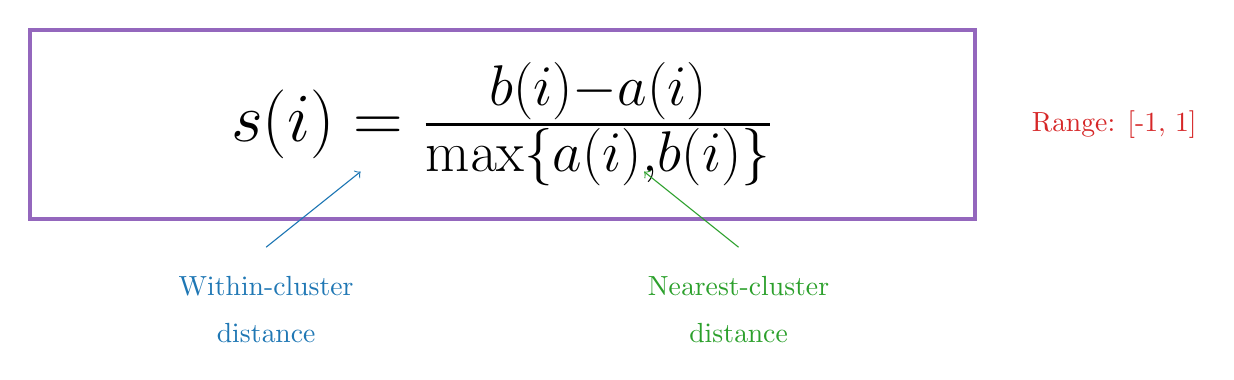
\begin{tikzpicture}[scale=1.2]
% Main formula box
\draw[ultra thick, mlpurple] (0,0) rectangle (10,2);
\node at (5,1) {\Huge $s(i) = \frac{b(i) - a(i)}{\max\{a(i), b(i)\}}$};

% Annotations
\node[mlblue, below] at (2.5,-0.5) {Within-cluster};
\node[mlblue, below] at (2.5,-1) {distance};
\draw[mlblue, ->] (2.5,-0.3) -- (3.5,0.5);

\node[mlgreen, below] at (7.5,-0.5) {Nearest-cluster};
\node[mlgreen, below] at (7.5,-1) {distance};
\draw[mlgreen, ->] (7.5,-0.3) -- (6.5,0.5);

\node[mlred, right] at (10.5,1) {Range: [-1, 1]};
\end{tikzpicture}
\end{center}

\vspace{1em}

\section*{Visual Intuition: Three Cases}

\begin{center}
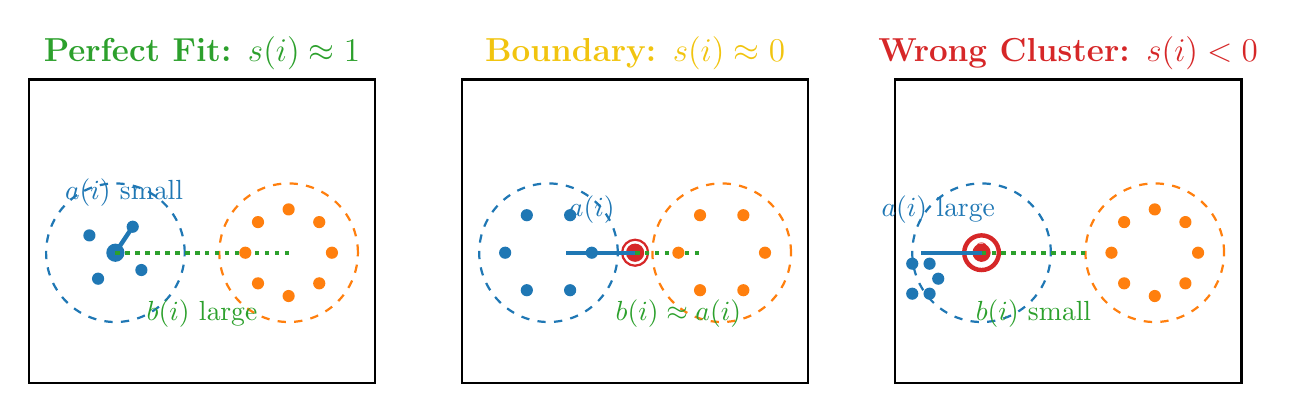
\begin{tikzpicture}[scale=1.1]
% Perfect fit: s(i) ≈ 1
\begin{scope}[shift={(0,0)}]
\draw[thick] (0,0) rectangle (4,3.5);
\node[font=\large\bfseries, mlgreen] at (2,3.8) {Perfect Fit: $s(i) \approx 1$};

% Draw clusters
\draw[mlblue, thick, dashed] (1,1.5) circle (0.8);
\draw[mlorange, thick, dashed] (3,1.5) circle (0.8);

% Point in blue cluster
\fill[mlblue] (1,1.5) circle (3pt);
\fill[mlblue] (0.7,1.7) circle (2pt);
\fill[mlblue] (1.3,1.3) circle (2pt);
\fill[mlblue] (0.8,1.2) circle (2pt);
\fill[mlblue] (1.2,1.8) circle (2pt);

% Show distances
\draw[mlblue, ultra thick] (1,1.5) -- (1.2,1.8);
\node[mlblue] at (1.1,2.2) {$a(i)$ small};

\draw[mlgreen, ultra thick, dotted] (1,1.5) -- (3,1.5);
\node[mlgreen] at (2,0.8) {$b(i)$ large};

% Orange cluster points
\foreach \angle in {0,45,90,135,180,225,270,315} {
    \fill[mlorange] (3,1.5) ++(\angle:0.5) circle (2pt);
}
\end{scope}

% Poor fit: s(i) ≈ 0
\begin{scope}[shift={(5,0)}]
\draw[thick] (0,0) rectangle (4,3.5);
\node[font=\large\bfseries, mlyellow] at (2,3.8) {Boundary: $s(i) \approx 0$};

% Draw clusters
\draw[mlblue, thick, dashed] (1,1.5) circle (0.8);
\draw[mlorange, thick, dashed] (3,1.5) circle (0.8);

% Boundary point
\fill[mlred] (2,1.5) circle (3pt);
\draw[mlred, thick] (2,1.5) circle (0.15);

% Show equal distances
\draw[mlblue, ultra thick] (2,1.5) -- (1.2,1.5);
\node[mlblue] at (1.5,2) {$a(i)$};

\draw[mlgreen, ultra thick, dotted] (2,1.5) -- (2.8,1.5);
\node[mlgreen] at (2.5,0.8) {$b(i) \approx a(i)$};

% Cluster points
\foreach \angle in {0,60,120,180,240,300} {
    \fill[mlblue] (1,1.5) ++(\angle:0.5) circle (2pt);
    \fill[mlorange] (3,1.5) ++(\angle:0.5) circle (2pt);
}
\end{scope}

% Wrong cluster: s(i) < 0
\begin{scope}[shift={(10,0)}]
\draw[thick] (0,0) rectangle (4,3.5);
\node[font=\large\bfseries, mlred] at (2,3.8) {Wrong Cluster: $s(i) < 0$};

% Draw clusters
\draw[mlblue, thick, dashed] (1,1.5) circle (0.8);
\draw[mlorange, thick, dashed] (3,1.5) circle (0.8);

% Misplaced point
\fill[mlred] (1,1.5) circle (3pt);
\draw[mlred, ultra thick] (1,1.5) circle (0.2);
\node[mlred] at (1,1.5) {?};

% Show distances
\draw[mlblue, ultra thick] (1,1.5) -- (0.3,1.5);
\node[mlblue] at (0.5,2) {$a(i)$ large};

\draw[mlgreen, ultra thick, dotted] (1,1.5) -- (2.2,1.5);
\node[mlgreen] at (1.6,0.8) {$b(i)$ small};

% Cluster points
\foreach \angle in {0,60,120,240,300} {
    \fill[mlblue] (0.3,1.2) ++(\angle:0.2) circle (2pt);
}
\foreach \angle in {0,45,90,135,180,225,270,315} {
    \fill[mlorange] (3,1.5) ++(\angle:0.5) circle (2pt);
}
\end{scope}
\end{tikzpicture}
\end{center}

\vspace{1em}

\section*{Cluster Quality Metrics Comparison}

\begin{center}
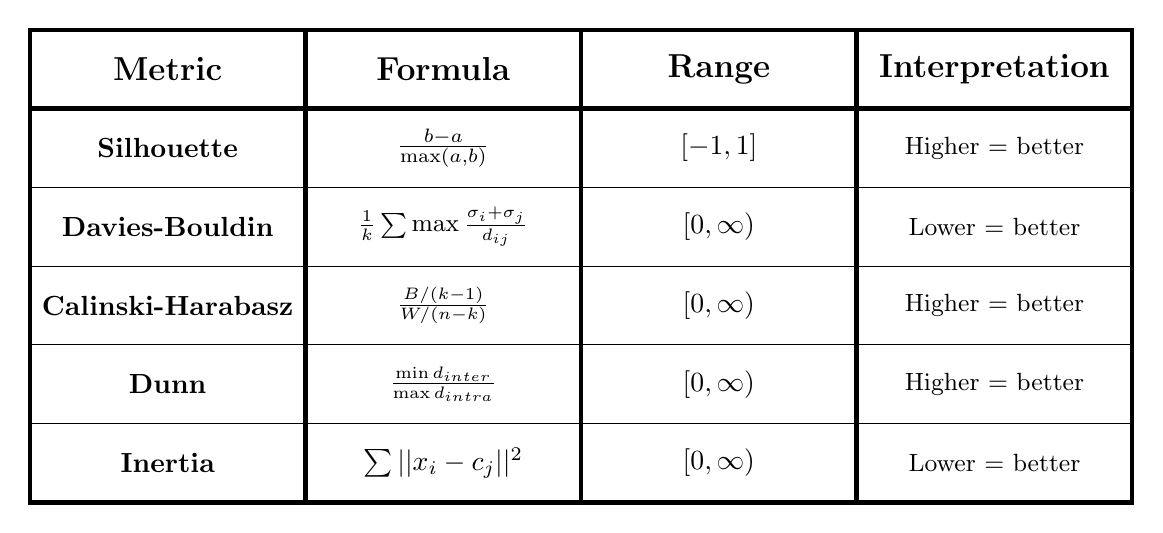
\begin{tikzpicture}[scale=1]
% Create comparison table
\draw[ultra thick] (0,0) rectangle (14,6);

% Headers
\draw[ultra thick] (0,5) -- (14,5);
\draw[ultra thick] (3.5,0) -- (3.5,6);
\draw[ultra thick] (7,0) -- (7,6);
\draw[ultra thick] (10.5,0) -- (10.5,6);

\node[font=\large\bfseries] at (1.75,5.5) {Metric};
\node[font=\large\bfseries] at (5.25,5.5) {Formula};
\node[font=\large\bfseries] at (8.75,5.5) {Range};
\node[font=\large\bfseries] at (12.25,5.5) {Interpretation};

% Silhouette
\draw (0,4) -- (14,4);
\node at (1.75,4.5) {\textbf{Silhouette}};
\node at (5.25,4.5) {$\frac{b-a}{\max(a,b)}$};
\node at (8.75,4.5) {$[-1, 1]$};
\node[font=\small] at (12.25,4.5) {Higher = better};

% Davies-Bouldin
\draw (0,3) -- (14,3);
\node at (1.75,3.5) {\textbf{Davies-Bouldin}};
\node[font=\small] at (5.25,3.5) {$\frac{1}{k}\sum \max \frac{\sigma_i + \sigma_j}{d_{ij}}$};
\node at (8.75,3.5) {$[0, \infty)$};
\node[font=\small] at (12.25,3.5) {Lower = better};

% Calinski-Harabasz
\draw (0,2) -- (14,2);
\node at (1.75,2.5) {\textbf{Calinski-Harabasz}};
\node[font=\small] at (5.25,2.5) {$\frac{B/(k-1)}{W/(n-k)}$};
\node at (8.75,2.5) {$[0, \infty)$};
\node[font=\small] at (12.25,2.5) {Higher = better};

% Dunn Index
\draw (0,1) -- (14,1);
\node at (1.75,1.5) {\textbf{Dunn}};
\node[font=\small] at (5.25,1.5) {$\frac{\min d_{inter}}{\max d_{intra}}$};
\node at (8.75,1.5) {$[0, \infty)$};
\node[font=\small] at (12.25,1.5) {Higher = better};

% Inertia
\node at (1.75,0.5) {\textbf{Inertia}};
\node at (5.25,0.5) {$\sum ||x_i - c_j||^2$};
\node at (8.75,0.5) {$[0, \infty)$};
\node[font=\small] at (12.25,0.5) {Lower = better};
\end{tikzpicture}
\end{center}

\newpage

\section*{Advanced: Average Silhouette Width}

\begin{center}
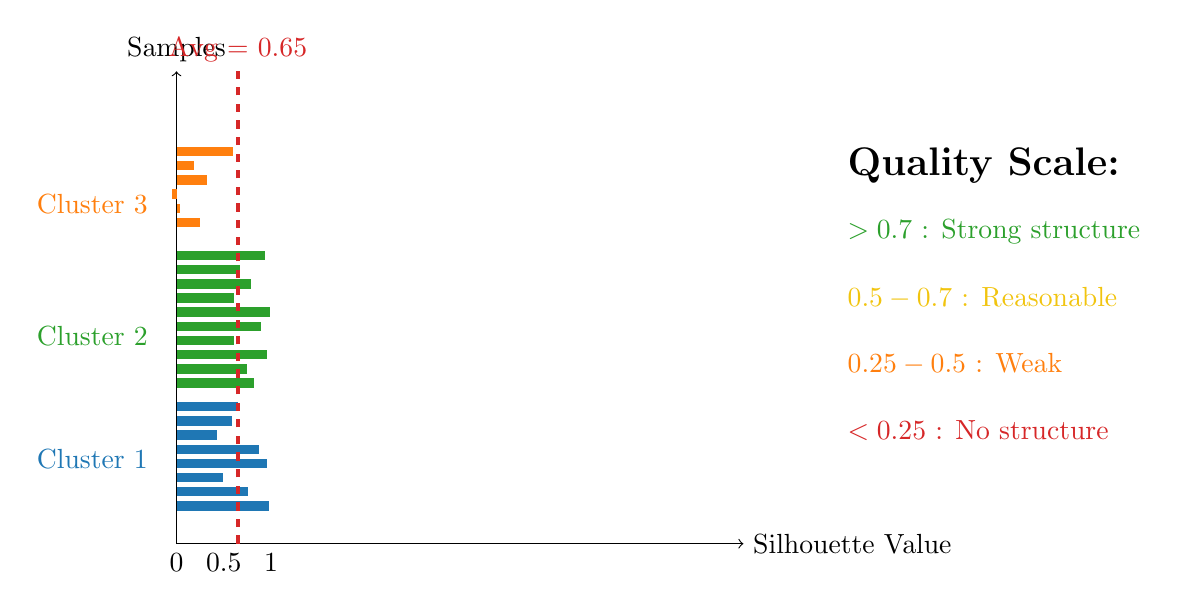
\begin{tikzpicture}[scale=1.2]
% Silhouette plot
\draw[->] (0,0) -- (6,0) node[right] {Silhouette Value};
\draw[->] (0,0) -- (0,5) node[above] {Samples};

% Draw silhouette bars for 3 clusters
% Cluster 1
\foreach \i in {1,...,8} {
    \pgfmathsetmacro{\width}{0.7 + rand*0.3}
    \fill[mlblue] (0,0.2+\i*0.15) rectangle (\width,0.3+\i*0.15);
}
\node[mlblue, left] at (-0.2,0.9) {Cluster 1};

% Cluster 2
\foreach \i in {1,...,10} {
    \pgfmathsetmacro{\width}{0.8 + rand*0.2}
    \fill[mlgreen] (0,1.5+\i*0.15) rectangle (\width,1.6+\i*0.15);
}
\node[mlgreen, left] at (-0.2,2.2) {Cluster 2};

% Cluster 3
\foreach \i in {1,...,6} {
    \pgfmathsetmacro{\width}{0.3 + rand*0.4}
    \fill[mlorange] (0,3.2+\i*0.15) rectangle (\width,3.3+\i*0.15);
}
\node[mlorange, left] at (-0.2,3.6) {Cluster 3};

% Average line
\draw[mlred, ultra thick, dashed] (0.65,0) -- (0.65,5);
\node[mlred, above] at (0.65,5) {Avg = 0.65};

% Scale
\foreach \x in {0,0.5,1} {
    \node[below] at (\x,0) {\x};
}

% Quality interpretation
\node[right, align=left] at (7,4) {\Large\textbf{Quality Scale:}};
\node[right, align=left, mlgreen] at (7,3.3) {$> 0.7$ : Strong structure};
\node[right, align=left, mlyellow] at (7,2.6) {$0.5 - 0.7$ : Reasonable};
\node[right, align=left, mlorange] at (7,1.9) {$0.25 - 0.5$ : Weak};
\node[right, align=left, mlred] at (7,1.2) {$< 0.25$ : No structure};
\end{tikzpicture}
\end{center}

\vspace{1em}

\section*{Discovery Challenge: Optimize k}

\begin{center}
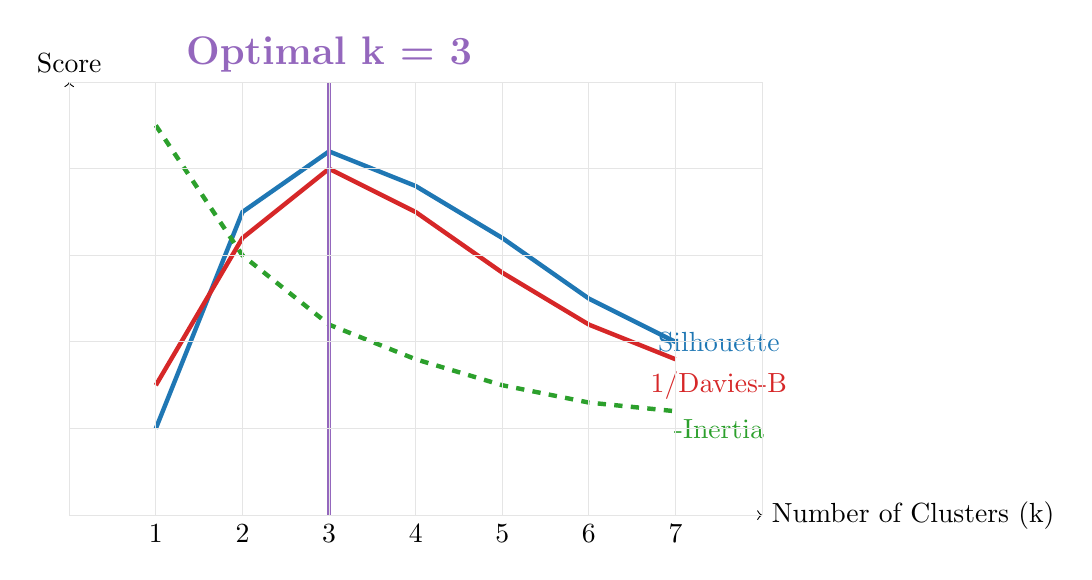
\begin{tikzpicture}[scale=1.1]
% Draw optimization curves
\draw[->] (0,0) -- (8,0) node[right] {Number of Clusters (k)};
\draw[->] (0,0) -- (0,5) node[above] {Score};

% Silhouette curve
\draw[mlblue, ultra thick] plot coordinates {(1,1) (2,3.5) (3,4.2) (4,3.8) (5,3.2) (6,2.5) (7,2)};
\node[mlblue] at (7.5,2) {Silhouette};

% Davies-Bouldin (inverted for comparison)
\draw[mlred, ultra thick] plot coordinates {(1,1.5) (2,3.2) (3,4) (4,3.5) (5,2.8) (6,2.2) (7,1.8)};
\node[mlred] at (7.5,1.5) {1/Davies-B};

% Inertia elbow
\draw[mlgreen, ultra thick, dashed] plot coordinates {(1,4.5) (2,3) (3,2.2) (4,1.8) (5,1.5) (6,1.3) (7,1.2)};
\node[mlgreen] at (7.5,1) {-Inertia};

% Optimal k
\draw[mlpurple, ultra thick] (3,0) -- (3,5);
\node[mlpurple, above] at (3,5) {\Large\textbf{Optimal k = 3}};

% k values
\foreach \k in {1,...,7} {
    \node[below] at (\k,0) {\k};
}

% Grid
\draw[gray!20, thin] (0,0) grid (8,5);
\end{tikzpicture}
\end{center}

\vspace{1em}

\section*{Your Investigation}

\begin{center}
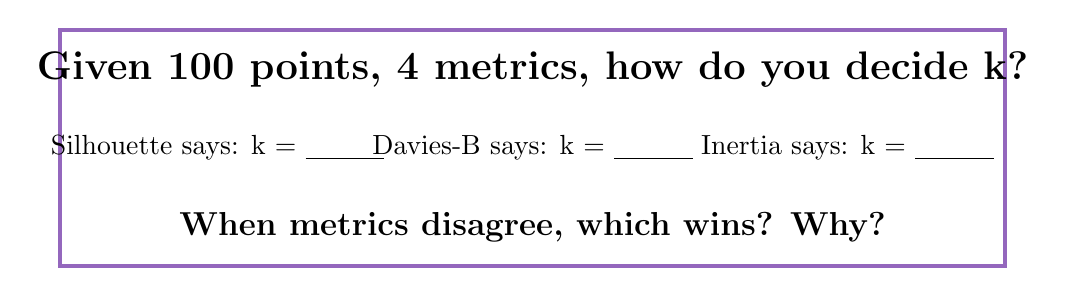
\begin{tikzpicture}[scale=1]
\draw[mlpurple, ultra thick] (0,0) rectangle (12,3);

\node[font=\Large] at (6,2.5) {\textbf{Given 100 points, 4 metrics, how do you decide k?}};

\node at (2,1.5) {Silhouette says: k = \underline{\hspace{1cm}}};
\node at (6,1.5) {Davies-B says: k = \underline{\hspace{1cm}}};
\node at (10,1.5) {Inertia says: k = \underline{\hspace{1cm}}};

\node[font=\large] at (6,0.5) {\textbf{When metrics disagree, which wins? Why?}};
\end{tikzpicture}
\end{center}

\vspace{1em}

\begin{tcolorbox}[colback=mlcyan!10, colframe=mlcyan!50]
\centering\large
\textbf{Next: DBSCAN} - When you don't know k at all!
\end{tcolorbox}

\end{document}